
%(BEGIN_QUESTION)
% Copyright 2012, Tony R. Kuphaldt, released under the Creative Commons Attribution License (v 1.0)
% This means you may do almost anything with this work of mine, so long as you give me proper credit

The flow of oily water from unit \#3 is shut off, but units \#1 and \#2 are still sending oily water at constant flow rates to this sump:

$$\includegraphics[width=15.5cm]{i0005rx01.eps}$$

FIR-140 shows a constant flow rate of 3.5 gallons per minute, and FIR-141 shows a constant flow rate of 4.1 gallons per minute.  At these flow rates, determine how long it will take for the oily water level inside the sump to accumulate from the low-level mark to the high-level mark, expressing the calculation using calculus notation.

\vskip 10pt

Sketch the graphical interpretation of this calculus problem, showing how a graph makes visual sense of the given information as well as the final result.

\underbar{file i01907}
%(END_QUESTION)





%(BEGIN_ANSWER)

We know we are given flow {\it rate} values in gallons per minute, and that the rise in liquid inside the sump equates to a certain volume in {\it gallons}.  We also are told to solve for time.  From this we know we can use {\it integration} to relate the variables together, because the time-integral of flow rate is volume (gallons per minute times minutes equals gallons).  

Let us set up a calculus expression using the variables $Q_1$ for FT-140's value of 3.5 GPM, $Q_2$ for FT-141's value of 4.1 GPM, $\Delta V$ for the accumulation of volume inside the sump, and $x$ for the unknown amount of time it will take for that much liquid to accumulate:

$$\Delta V = \int_0^{x} (Q_1 + Q_2) \> dt$$

We know the total volume of the sump is 35000 gallons, and that is at a liquid height of 8 feet 11 inches (8.91667 feet).  This means each foot of depth is equivalent to 3925.23 gallons (assuming a constant width and length of the sump at all liquid levels.  The difference in depth between the high and low level marks is 4 feet 6 inches (4.5 feet), which equates to 17663.55 gallons.  This will be our $\Delta V$ value.

Combining the flow rates $Q_1$ and $Q_2$ (3.5 GPM + 4.1 GPM = 7.6 GPM) and plugging in our known value of 17663.55 gallons for $\Delta V$:

$$17663.55 \hbox{ gal} = \int_0^{x} (7.6 \hbox{ gal/min}) \> dt$$

The graphical interpretation of integration is the {\it area} bounded by a function.  In this case, the function being integrated is a constant total flow rate of 7.6 GPM (a horizontal line on a graph, with flow as the vertical axis and time as the horizontal axis):

$$\includegraphics[width=15.5cm]{i01907x01.eps}$$

Simple division tells us the required width of this area: {\bf 2324.15 minutes}, or {\bf 38 hours and 44.15 minutes}.

\vskip 10pt

\filbreak

Another way we could have solved for the unknown time is to use {\it differentiation}.  The total flow rate of liquid into the sump (7.6 GPM) could be expressed as a {\it derivative} of volume with respect to time:

$${dV \over dt} = 7.6 \hbox{ gallons per minute}$$

Since we happen to know this flow rate is constant (not changing), we may conclude that the {\it difference quotient} of the entire change in volume over the span of time it takes to accumulate that volume will also have the same value:

$${\Delta V \over \Delta t} = {17663.55 \hbox{ gallons} \over x \hbox{ minutes}} = 7.6 \hbox{ gallons per minute}$$

The graphical interpretation of differentiation is the {\it slope} of a function.  In this case, the function being integrated is a constant total flow rate of 7.6 GPM (a horizontal line on a graph, with flow as the vertical axis and time as the horizontal axis):

$$\includegraphics[width=15.5cm]{i01907x02.eps}$$

$${\Delta V \over \Delta t} = {dV \over dt} = {17663.55 \hbox{ gallons} \over x \hbox{ minutes}} = {7.6 \hbox{ gallons} \over 1 \hbox{ minute}}$$

Once gain, simple division tells us the required $\Delta t$ or $x$ value: {\bf 2324.15 minutes}, or {\bf 38 hours and 44.15 minutes}.

%(END_ANSWER)





%(BEGIN_NOTES)

\vskip 20pt \vbox{\hrule \hbox{\strut \vrule{} {\bf Virtual Troubleshooting} \vrule} \hrule}

This question is a good candidate for a ``Virtual Troubleshooting'' exercise.  Presenting the diagram to students, you first imagine in your own mind a particular fault in the system.  Then, you present one or more symptoms of that fault (something noticeable by an operator or other user of the system).  Students then propose various diagnostic tests to perform on this system to identify the nature and location of the fault, as though they were technicians trying to troubleshoot the problem.  Your job is to tell them what the result(s) would be for each of the proposed diagnostic tests, documenting those results where all the students can see.

During and after the exercise, it is good to ask students follow-up questions such as:

\begin{itemize}
\item{} What does the result of the last diagnostic test tell you about the fault?
\item{} Suppose the results of the last diagnostic test were different.  What then would that result tell you about the fault?
\item{} Is the last diagnostic test the best one we could do?
\item{} What would be the ideal order of tests, to diagnose the problem in as few steps as possible?
\end{itemize}

%INDEX% Mathematics, calculus: integral (calculating volumes from measured flow rates at specific times)
%INDEX% Process: oily water sump (realistic P&ID shown)

%(END_NOTES)

